\documentclass{sciposter}
\usepackage[dvipsnames,usenames,svgnames,table,x11names, rgb, html]{xcolor} 
\usepackage{lipsum}
\usepackage{epsfig}
\usepackage{amsmath}
\usepackage{amssymb}
\usepackage[german]{babel}
\usepackage{geometry}
\usepackage{multicol}
\usepackage{graphicx}
\usepackage{tikz}
\usepackage{wrapfig}
\usepackage{gensymb}
\usepackage[utf8]{inputenc}
\usepackage{empheq}
\usepackage{mathpazo}
\usepackage[T1]{fontenc}
\renewcommand{\familydefault}{\rmdefault}
\usepackage{eulervm}

% for nice tableas
\usepackage{booktabs}

% so we have more space between matrix entries
\setlength{\arraycolsep}{12pt}

\geometry{
 landscape,
 a1paper,
 left=5mm,
 right=50mm,
 top=5mm,
 bottom=50mm,
 }


\usepackage{todonotes}

\newcommand{\nnz}{d\operatorname{nnz}}
\newcommand{\TODO}[1]{\todo[inline, color=red!40]{#1}}
\renewcommand{\vec}[1]{\mathbf{#1}}
%BEGIN LISTINGDEF



\usepackage{listings}
\usepackage{inconsolata}


\usepackage{mdframed}

\newenvironment{method}[1]{\begin{mdframed}[backgroundcolor=blue!10,innertopmargin=15pt, innerbottommargin=15pt, nobreak=true]
		\textbf{#1 }
	}
	{ 
	\end{mdframed}
}

\newenvironment{important}{\begin{mdframed}[backgroundcolor=red!50,innertopmargin=15pt, innerbottommargin=15pt, nobreak=true]
		\Large
	}
	{ 
	\end{mdframed}
}

\newenvironment{trick}[1]{\begin{mdframed}[backgroundcolor=PineGreen!50,innertopmargin=15pt, innerbottommargin=15pt, nobreak=true]
			\textbf{#1 }
	}
	{ 
	\end{mdframed}
}


\definecolor{background}{HTML}{FAFAFA}
\definecolor{comment}{HTML}{ABB0B6}
\definecolor{keywords}{HTML}{55B4D4}
\definecolor{basicStyle}{HTML}{6C7680}
\definecolor{variable}{HTML}{001080}
\definecolor{string}{HTML}{86B300}

\newcommand{\norm}[1]{\left\lVert#1\right\rVert}


\lstset{
	% How/what to match
	sensitive=true,
	% Border (above and below)
	frame=single,
	% Extra margin on line (align with paragraph)
	xleftmargin=\parindent,
	% Put extra space under caption
	belowcaptionskip=1\baselineskip,
	% Colors
	backgroundcolor=\color{background},
	basicstyle=\color{basicStyle}\ttfamily,
	keywordstyle=\color{keywords},
	commentstyle=\color{comment},
	stringstyle=\color{string},
	numberstyle=\color{sviolet},
	identifierstyle=\color{variable},
	% Break long lines into multiple lines?
	breaklines=true,
	% Show a character for spaces?
	showstringspaces=false,
	tabsize=2
}

%END LISTINGDEF


\newcommand*\widefbox[1]{\fbox{\hspace{2em}#1\hspace{2em}}}


\newlength\dlf  % Define a new measure, dlf
\newcommand\alignedbox[2]{
% Argument #1 = before & if there were no box (lhs)
% Argument #2 = after & if there were no box (rhs)
&  % Alignment sign of the line
{
\settowidth\dlf{$\displaystyle #1$}
    % The width of \dlf is the width of the lhs, with a displaystyle font
\addtolength\dlf{\fboxsep+\fboxrule}
    % Add to it the distance to the box, and the width of the line of the box
\hspace{-\dlf}
    % Move everything dlf units to the left, so that & #1 #2 is aligned under #1 & #2
\boxed{#1 #2}
    % Put a box around lhs and rhs
}
}
\usepackage{graphicx,url}
\usepackage{tabularx}

%BEGIN TITLE
\title{\huge{Data Modelling and Databases}}

% if you want to set an author replace the next line with \author{your name here}
\author{David Bohner}



\begin{document}
\fontfamily{lmss}\selectfont
\maketitle

\begin{multicols}{3}

\section{Key Definitions}
\begin{tabularx}{\linewidth}{r X}
\textbf{Database} & A collection of data\\
\textbf{DBMS} & Database Management System\\
\textbf{Instance} & TODO\\
\textbf{Query} & A function that takes a DB instance as input and outputs a new relation
\end{tabularx}
\subsection{DBMS}
\begin{mdframed}
\subsubsection{A DBMS Provides:}
\begin{tabularx}{\linewidth}{r|X}
Data Independence & App. should \underline{not} know how data is stored\\
Efficient Data Storage\\
Transactional Access & \underline{As if} there was only a \underline{single user} using a system \underline{that never fails}\\
Generic Abstraction & Users don't need to worry about the above with each new query
\end{tabularx}
\end{mdframed}

\begin{mdframed}
\subsubsection{Potential \underline{Downsides} of a DBMS}
\begin{tabularx}{\linewidth}{r|X}
Workload Mismatch & App is not what DBMS is designed for\\
Data Model Mismatch & Data required cannot be modelled by the DBMS \textit{(e.g. a graph, while DBMS can only provide tables)}
\end{tabularx}
\end{mdframed}

\section{DB Models}
\subsection{IMS/Hierarchical}
\subsection{Network Model}
\subsection{Relational Model}
\subsubsection{Schema}
\section{Queries: Relational Algebra}
\begin{method}{Set Operations}\\
\begin{tabularx}{\columnwidth}{r|X}
Union $\cup$ & $x \in R_1 \cup R_2 \iff x \in R_1 \lor x \in R_2$\\
Difference $-$ & $x \in R_1 - R_2 \iff x \in R_1 \land \lnot (x \in R_2)$\\
Intersection $\cap$ & $x \in R_1 \cup R_2 \iff x \in R_1 \land x \in R_2$\\
Selection $\sigma$ & $x \in \sigma_c(R) \iff x \in R \land c(x) = \text{True}$\\
Projection $\Pi$ & $\Pi_{A_1,...,A_n}(R)$ only keeps a subset of columns.\\
Cartesian Product $\times$ & $(x, y) \in R_1 \times R_2 \iff x \in R_1 \land y \in R_2$\\
Renaming $\rho$ & $\rho_{B_1,...,B_n}(R)$ change the name of attributes in $R$ to $B_1, ..., B_n$\\
Natural Join $\bowtie$ & $R_1(A, B) \bowtie R_2(B, C) = \Pi_{A, B, C}(\sigma_{R_1.B=R_2.B}(R_1 \times R_2))$\\
Theta Join $\bowtie_\theta$ & $R_1 \bowtie_\theta R_2 = \sigma_\theta(R_1 \times R_2)$\\
Equi-Join $\bowtie_{A=B}$ & $R_1 \bowtie_{A=B} R_2 = \sigma_{A=B}(R_1 \times R_2)$
\end{tabularx}
\end{method}
\begin{mdframed}
\subsection{Natural Join Special Cases}
\textbf{Case 1: No shared attributes}\\
$R(A, B, C), S(D, E): R \bowtie S = R \times S$\\
\textbf{Case 2: Share all attributes}\\
$R(A, B, C), S(A, B, C): R \bowtie S = R \cap S$
\end{mdframed}
\subsection{Presenting Operations Graphically}
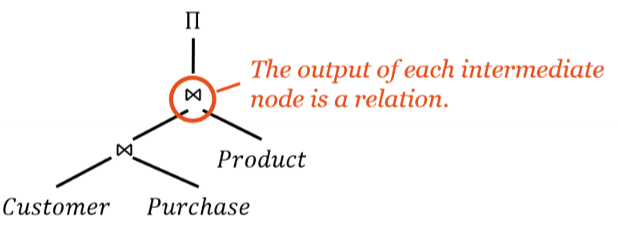
\includegraphics[width=\columnwidth]{images/relational_algebra_tree.png}

\end{multicols}
\end{document}